\documentclass[]{msulabm}
\usepackage[utf8]{inputenc}
\usepackage{amsmath}
\usepackage{graphicx}
%\usepackage[linktocpage]{hyperref}  % if not using colorlinks, use linktocpage
\usepackage[colorlinks]{hyperref}  % if not using colorlinks, use linktocpage
\usepackage{bm}            % bold math
\usepackage{multirow}
\usepackage[table]{xcolor} % provide alternating rows with colors
\usepackage{textcomp}
\usepackage{xfrac} % gives split-level fractions with '\sfrac{a}{b}
\usepackage{multicol}
\usepackage[section]{placeins} % provides \FloatBarrier, to keep floats from crossing this barrier
\usepackage{amssymb}
\usepackage{wrapfig} % provides wrapping figures with text.
%\usepackage{enumitem} % gives \begin{enumerate}[resume] to resume counting from previous enumerate
%\usepackage{subfigure}
%\usepackage{tikz} % to draw arrows
\usepackage{xtab} % provides xtabular, tabular environment that spans multiple pages and other awesome things
\usepackage[style=phys,biblabel=brackets,pageranges=false]{biblatex}
\usepackage{pdflscape}
\usepackage{ragged2e}
\usepackage{longtable}

\bibliography{references-manual,bbarker-zotero}

\newcommand{\abs}[1]{\left\lvert#1\right\rvert}

\title{Laboratory Manual}
\author{PHSC 12700 Stars \\ \\ The University of Chicago}
\date{Autumn 2019}

\pagestyle{ruled}

\definecolor{lgray}{rgb}{.2,.2,.2}

\makeevenfoot{ruled}{\thepage}{\footnotesize{\textit{Last updated \today}}}{}
%\makeevenfoot{ruled}{\thepage}{}}{}
\makeoddfoot{ruled}{}{\color{lgray} \tiny{This work is licensed under \href{http://creativecommons.org/licenses/by-sa/4.0/}{CC BY-SA 4.0} by \href{mailto:bbarker@uchicago.edu}{the University of Chicago}.}}{\thepage}


% allows us to use subcaptions from the memoir class in figures. See Memoir Section 10.9
\newsubfloat{figure}

% don't worry so much about filling every page.
%\raggedbottom

% raise the penalty for splitting footnotes across different pages. Default is 100.
\interfootnotelinepenalty=10000

%\includeonly{amplifier/amplifier} 

% creates a standard length to use 
\newlength{\answerskip}
%\setlength{\answerskip}{90pt} 

%% use plus / minus if latex is squeezing the answer space too much
\setlength{\answerskip}{2cm plus 0.2cm minus 0.2cm}

\newlength{\qaskip}
\setlength{\qaskip}{\answerskip}
\addtolength{\qaskip}{\baselineskip}

% reduce vertical space between chapters in table of contents. Default is 2em.
\setlength{\cftbeforechapterskip}{1em}

% allow for extra line on a page to help prevent widow/orphan lines.
\sloppybottom

% Now we can caption a table outside of the table float environment (good for multi-page tables)
\newfixedcaption{\freetabcaption}{table}

%\includeonly{snells-law/snells-law}
%\includeonly{ohms-law/ohms-law}

\begin{document}
\maxtocdepth{chapter}

 % start roman numbering
 \frontmatter

\maketitle

%\clearpage

%Brent W. Barker

%Department of Astronomy \& Astrophysics

%The University of Chicago

%5640 South Ellis Ave.

%Chicago, IL 60637

%\href{mailto:bbarker@uchicago.edu}{bbarker@uchicago.edu}

%\vspace{2\baselineskip}

%\includegraphics{cc-by-sa-88x31}

%\textcopyright{} 2018 Brent W. Barker. Except where otherwise noted, this work is copyrighted under the Creative Commons Attribution-ShareAlike International 4.0 License. To view a copy of this license, visit \url{http://creativecommons.org/licenses/by-sa/4.0/}.

%\vspace{\baselineskip}

 % skip to next right leaf (``recto'')
 \cleartorecto

 % the star means that the ToC itself is not listed in the ToC
 \tableofcontents*

 % start arabic numbering
\mainmatter 

\chapter{Bending light to see into space}

Optical telescopes are one way that astronomers use to better observe the cosmos. In this lab, you will build up your understanding about how telescopes help us do this.

\section{Learning Goals}

\begin{itemize}
	\item Learn how light behaves when traveling between mediums.
	
	\item Create an image with a lens.
	
	\item Configure a refracting telescope and explain how it helps for observing the sky.
\end{itemize}

\section{But first! Observing with Stone Edge Observatory}

Throughout the quarter, you will be taking data (images) with a robotic telescope that is located in Sonoma, California. This week, you will select a target and queue some images to be taken.

\section{How do we use materials to bend light?}

We use lenses all the time to shape the path that light takes, either with eyeglasses or with optical telescopes. These activities are intended to help you understand how we use materials to bend light.

\begin{steps}
	\item Find the ray box and a trapezoidal prism in your kit. Set the prism on a white sheet of paper and adjust the ray box so that it is shining 1 ray of line from the side and onto the prism. Play with the angle at which the ray strikes the prism and observe what happens to the light ray that extends into the prism. How does the path of the ray change when it enters the prism? \textbf{Record your observations. Be specific about any patterns you notice.}
	
	\item It's hard to see the light in the prism, so let's use a simulation. Go to \url{https://phet.colorado.edu/en/simulation/bending-light} and select the play button to launch the simulation. Select the leftmost ``Intro'' box. This is a side view of the interface between two materials, currently air on the top half of the screen and water on the bottom. A laser is positioned above the interface.
	
	\item Play with the controls on this screen until you have an idea of how to move the laser, turn it on and off, and adjust the materials on the top and bottom. To reset the simulation, select the orange circular button on the lower right.
	
	\item Observe what happens to the laser beam when you change the angle, materials, and indices of refraction. \textbf{Record your observations for your lab report.} For example, ``when the angle between the laser and the interface gets smaller, the laser gets deflected more/less''.

	\item Open the second screen at the bottom of the sim. Lenses are wider in the middle and thinner at the top and bottom, so drag a triangle up and shine a ray through it. Then bring a second triangle up, rotate it upside down, and arrange the two so they look a bit like a convex lens. Set the laser to output several parallel rays and aim it so some of the rays hit the top triangle and some hit the bottom triangle. \textbf{Record your observations.}
	
	\item Go back to your physical ray box and optics set. Adjust the ray box to emit 5 parallel rays and set up the convex lens (the one that is thinner on the ends and thicker in the middle) so that the rays are hitting it from the side. Notice where the rays go after they go through the lens. \textbf{Record your observations.}
\end{steps}

This setup of parallel rays is convenient for seeing precisely what the lens does. It also happens to be the situation when we observe things that are very far away compared to length scales of the lens. Consider two stakes driven into the ground next to each other, both perpendicular to the ground (and thus pointing directly at the center of the Earth). Since the Earth is a sphere, those stakes can't actually be both pointing directly toward the center of the Earth and also parallel to each other. For the former to be true, they must be angled slightly away from each other. But since the distance between them is so short compared to the distance away from the Earth's center, they are effectively parallel. \textit{This is the same with light arriving from distant objects like stars.}

\begin{steps}
	\item Let's try putting some parallel rays from a distant object on a lens and see what happens where those rays intersect. Take one of the round lenses in a black plastic lens holder and shine those parallel rays from the light box on it to find the distance where the rays intersect.
	
	\item Select a distant bright object with sharply contrasting edges, like a building outside the window during the daytime, an exposed florescent bulb, or the light-up target on the other side of the ray box. Hold the lens between the object and a white sheet of paper. The white sheet of paper should be placed about the same distance away as the intersection distance. \textbf{Record your observations.}
\end{steps}

This intersection distance is called the ``focal length'' of the lens, and if an object is a long distance away compared to the focal length, then its image is formed at the focal length (if the object is closer, the the image is formed further away than the focal length).

This principle works in reverse too --- if an object is placed at the focal length of the lens, the rays come out parallel on the other side. The image is effectively formed an infinite distance away.

\begin{steps}
	\item Design and conduct an experiment to find the focal length of the lens you just used. Decide as a group how to measure, and how to estimate an uncertainty for your measurement. See Appendix\ \ref{cha:uncertainty} for detailed information about estimating uncertainty. \textbf{Record a sketch of your setup, a description of your procedure for gathering and analyzing your data, and the data itself.}

	\item Compare: how does this focal length compare to the focal length that is printed on the lens holder? See Appendix\ \ref{unc:sec:comparing} for how to compare two values, taking into account their uncertainties. \textbf{Record this comparison calculation and what you conclude about how close they are. Is the printed value correct?}
\end{steps}

This lens setup is great for producing images, for example to record onto photographic film or a digital camera's image sensor. It's less good for look through, to magnify and gather more light the way we want to with a telescope. For that, we'll need at least two lenses.

\section{Your first telescope}

Telescopes come in many different configurations. Here you'll construct one that is simple by comparison, a refracting telescope, using just 2 lenses.

\begin{steps}
	\item Here's the principle for building this telescope: the image created by the first lens, called the objective lens, is the object for the second lens, which is called the eyepiece lens. The thing we are wanting to look at (the object for the objective lens) is far away. We want the image created by the eyepiece lens to be an infinite distance away on the near side (just trust me on this). \textbf{Given these design goals and the information about lenses above, where should the two lenses be positioned with respect to each other? Sketch your proposal, labeling each lens and drawing the focal lengths of each lens.}
	
	\item Using the optical bench, construct and test your telescope. Look at a distant (across the room) object through it. If you don't get a clean image of it by looking through the eyepiece lens, iterate on your design until you get it.
	
	\item Find the magnification of your telescope. Hint: if you have two identical objects, how close does one need to be to look the same size/distance as the one you see through the telescope? Experimentally determine this magnification factor (1 is no magnification, 2 means it looks twice as close, etc), and estimate the uncertainty of your magnification. \textbf{Record this.}
	
	\item Magnification should be related to the properties of the two lenses. Make up a formula that relates the focal lengths of your lenses to the magnification of your telescope. You may need to switch the lenses around or use different ones to test your formula. \textbf{Record this.}
\end{steps}

\section{Report checklist and grading}

Each item below is worth 10 points, and there is an additional 10 points for attendance and participation. See Appendix\ \ref{cha:lab-report-format} for guidance on writing the report and formatting tables and graphs.

\begin{itemize}
	\item Detailed observations from Steps 1--8.
	
	\item Sketch of your setup and procedure for finding the focal length in Step 9, as well as value, with uncertainty, of the focal length.
	
	\item Comparison of your measured focal length to the manufacturer's stated focal length, from Step 10.
	
	\item Detailed sketch of your working telescope design, from Steps 11--12.
	
	\item Experimental determination of the magnification of your telescope, with uncertainty.
	
	\item Formula relating the focal lengths to the magnification.
	
	\item Discuss the findings and reflect deeply on the quality and importance of the findings. This can be both in the frame of a scientist conducting the experiment (``What did the experiment tell us about the world?'') and in the frame of a student (``What skills or mindsets did I learn?'').
	
\end{itemize}
\chapter{Answering questions with astronomical images}

Last week, you queued up some images to be taken by the robotic telescope and learned how telescopes work to create images. This week, you'll learn how we record these images, and you'll learn one way to analyze those images to create knowledge about the distance between stars.

\section{Learning goals}

\begin{itemize}
	\item Answer questions by analyzing data that you took yourself.
	
	\item Experience and analyze the light gathering and angular resolution benefits of telescopes.
	
	\item Use pixel scale and length measurements to determine the angular separation of objects in a digital image.
	
	\item Gain insight of and appreciation for the scale of astronomical distances.
\end{itemize}

\section{How big is your face?}

This is a simple question, so that you can learn some astronomical concepts and tools while answering it and still keeping the subject matter intuitive.

\subsection{Background: reflecting telescopes and CCDs}

The primary utility of a telescope is its ability to gather light, thereby enabling visualization and analysis of the faint astronomical objects we are trying to observe. This requires focusing light incident on a large surface area. We will be using a \textbf{reflecting} telescope, which means that light rays from observation targets are focused into an eyepiece or onto a detector with reflecting mirrors. This is in contrast to refracting telescopes, which use refracting lenses to focus light rays. Figure~\ref{sot:fig:schmidt} shows schematically how this kind of telescope works. 

\begin{figure}
	\centering
	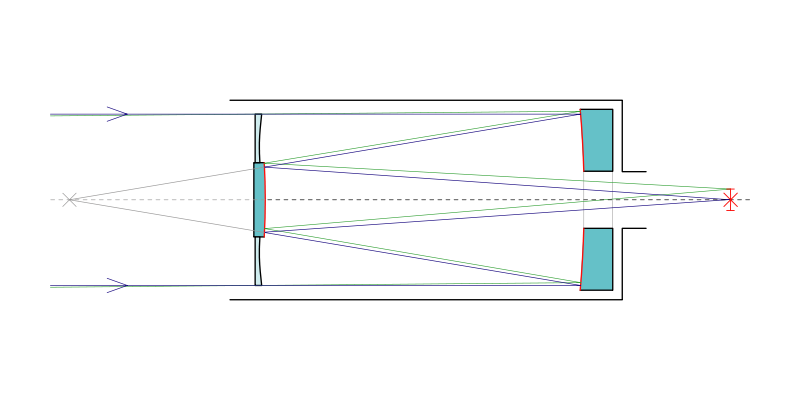
\includegraphics[scale = 0.5]{small-optical-telescopes/Schmidt-Cassegrain-Telescope.png}
	\caption{Schematic for a reflecting telescope of a Schmidt-Cassegrain design. 
		Light rays from astronomical objects enter the telescope in parallel because their source is effectively at infinity. They are then reflected by a parabolic primary mirror onto a secondary mirror that again reflects the light to a focus. An eyepiece or a camera is placed at the focal plane of the resulting image. Image source: \url{https://en.wikipedia.org/wiki/Cassegrain\_reflector\#/media/File:Schmidt-Cassegrain-Telescope.svg}}\label{sot:fig:schmidt}
\end{figure}

To take images in this lab, and to observe astronomical objects using the SEO, we make use of a \textbf{Charge Coupled Device (CCD)}. CCDs are the standard detectors for taking astronomical images at wavelengths blueward of approximately 1 micron. Think of the CCD we are using as a
very advanced low-noise digital detector, not wholly dissimilar from the digital detector in your
smartphone. Every time a photon within a certain energy range hits the detector, an electron is knocked off of the incident pixel, charging that pixel's capacitor. Thus, for each pixel, more photons $\implies$ more electrons $\implies$ more charge, and the charge can be read off into a digital signal that is then processed as an image. 

The main thing to note is that the CCD material is not sensitive to all wavelengths of light uniformly. Photons of certain energies are more likely to excite electrons in the detector and thus contribute to the output image. Consequently, the observed image intensity will be weighted by the response function of the detector.

\subsection{Telescope Set Up, Preliminary Observations}\label{ai:sec:setup}

The telescope and camera assembly is an expensive and relatively fragile piece of hardware, so
move carefully when interacting with the system. We have only two setups, so the class will be split into two groups for using the classroom telescope.

First we will be observing an object at the opposite end of the lab room with the lights turned off. During this exercise we will 1) check that the telescope is focused (which should already be the case), 2) gain practice positioning the telescope and targets, and 3) demonstrate the light gathering and angular resolution capabilities of the telescope with a physical object for which you have an direct sense of scale. \textbf{NOTE: For safety purposes, do not walk around the
	lab while the lights are off; instead, turn the lights off only as needed to gather data
	or make observations, and when the lights are off, don’t move about significantly.}

\begin{steps}
	\item The telescope should already be set up, with the camera on and cooled, and be approximately
	in focus and pointed at the target at the other end of the lab bench. If not, your TA will
	work with you to get the setup roughly correct.
	
	\item Your first task will be to tweak the centering of the image target. This doesn’t have to be
	perfect, but you should be able to see the mm scale marks. The telescope can be moved in elevation (up-down). The fine control of elevation is achieved using a knob on the mount - your TA will show you details. To shift the image left or right, move the target instead.
	
	\item Next we want to precisely focus the telescope. Do this with most of the lights off --- otherwise
	the image has too much light. Use the 4th filter of the five available; this can be selected
	from the ‘Filter’ menu. Then, use the \textbf{Focus} task from the camera control system toolbar,
	and take images of a few seconds (at most). If the image is completely dark, and the peak intensity number in the focus box is reading around 65000, then the CCD is saturated, and the light in the room should be reduced, or the exposure time shortened.
	
	\item Start the focus sequence - the camera will just
	take and display images repeatedly, of the exposure duration you specified. Now, adjust
	the focus knob (on the back of the telescope, off center) until you achieve an optimal focus.
	Note that you can (and should) zoom the magnification of the image so you can see the
	imaging target in detail. Do this by adjusting the magnification, and adjusting the image
	x,y centering so you’re looking at an appropriate zoomed location in the image. Note that
	you’ll need to not be touching the telescope or mount to get a sharp image, so you’ll
	have to adjust, then move away, wait, and repeat. Your classmates walking around the lab
	will cause image shake that will make focusing difficult, so enforce a still classroom while
	you do this.

	\item Once the telescope is focused, \textbf{grab a 1-second exposure} using the Grab command.
	
%	\item Time to demonstrate one helpful aspect of telescopes by taking an image in the dark. Once the telescope is focused to the sharpest possible images, turn off the lights and acquire an image using the
%	\textbf{Grab} button on the toolbar. An exposure time of 40--60 seconds is usually good with all of
%	the lab lights off and the blinds closed.
	
	\item Save this image in ‘fits’ format; the ‘ds9’ tool available on all of the lab
	computers can be used to examine the image in detail (you can also install this free software on your computer). You can use the university supported
	’Box’ system to share data with your lab classmates (or any other filesharing app that you prefer). See \url{uchicago.account.box.com/login}
	for details.
	
%	\item With the lights back on, gather around the target on the lab bench and then
%	turn the light off again. Observe the target. Can you see it? Can you see the details? Does
%	it matter how close you are (Rubric Row B5)?
%	
%	\item Compute and report the ratio of the light gathering power of
%	the telescope relative to your eye, and comment on how that relates to what you do (or do
%	not) observe by eye compared to the telescope (Rubric Row B9).

	\item Load the image in DS9. You can adjust the contrast of the image by holding down the right-click and dragging left, right, up, and down. In the upper right window, you can drag the frame around to view different parts of the image. To measure a length, select Region $>$ Shape $>$ Ruler from the drop-down menu. Then select Edit $>$ Region. Now if you click and drag on the image, it will draw a line and display the distance in pixels, or in angular separation if the image file has been calibrated withe pixel scale already.
	
	\item In the acquired and saved image you can see a mm scale, which correponds to some number
	of pixels. Compute and report the ‘pixel scale’ in mm/pixel. Given the distance between the
	telescope and the target, what is the angular pixel scale in arcseconds/pixel?
	
	To find this, note that for an arc (segment) of a circle, the length of that arc $s$ is related to the radius of circle $r$, and the angle (in radians) subtended by that arc $\theta$ by
	\begin{equation}
	s = r \theta
	\end{equation}

	\item Based on the pixel scale alone, how far apart in angle would two stars need to be in order to be distinguished as two objects instead of one?
	
	\item Observe the target from the vantage
	point of the telescope by eye. What detail can you see? How does that compare to what
	you can see with the telescope?
	
	\item Now take an image of part of one of your groupmates with the telescope. Centering on their eye can make for a fun picture. Use the pixel scale that you determined, along with that image, to find the angular separation (or ``angular distance'') between two points in the image --- for example, what is the angle subtended by their eye? Use the distance from the telescope to the person to also determine the distance between those two points, for example in millimeters. %Estimate your uncertainty and compare this measurement to a direct one (by holding up a ruler, for example.)
\end{steps}

\section{How far apart are these stars?}

Now that you have experience measuring distances for objects you can directly measure, you'll try your hand at measuring distant objects that none of us can measure directly --- other stars in your image from SEO! The goal here is to pick two stars in your image and find the angular separation between them, as well as physical distance. To get the physical distance, you'll need to know their distances from Earth. To get that, you'll need to match up those stars in your image to known stars. You can use Stellarium for this, a free virtual observatory app. Then you can select those stars in the app and easily find information about them.

Note that since we are using a real robotic telescope, many things can go wrong that may result in you not having an image that you've taken. There could have been cloudy nights all week, or smoke from wildfires, or planned power outages to protect from wildfires, or part of the observatory could have broken down. We have archival images in the case that your images are not taken, so that you can still complete the lab.

\begin{steps}
	\item Log into \url{queue.stoneedgeobservatory.com}, find your completed observation, and click ``go to image''. If you don't have a completed observation, find a classmate's or TA's image URL to visit to get an image to work with. If the image that appears is very fuzzy or has no stars in it, choose a different option from the ``Pipe Step'' drop-down menu.
	
	\item Select the link ``Download Selected FITS File'' to do so. Open it in DS9.
	
	\item Also open Stellarium on a computer. It is a free open source virtual observatory, so you can install it on your computer if you'd like. Use Stellarium to find your target (hover over the left edge of the screen to find the menu that includes the Search function). Toggle the Ground and Atmosphere in the bottom menu, so you can see the star clearly. Zoom in by selecting the rectangle icon third from the right in the upper-right-hand corner. This simulates a field of view that is similar to our telescope.
	
	\item Use the Stellarium view to identify two stars from your image. The two pictures might be rotated relative to each other.
	
	\item For those two stars, use DS9 to measure the angular separation (angular distance) between them. You may need to use the pixel scale of the Stone Edge Observatory telescope, which is 0.76''/pix (arcseconds per pixel). \textbf{Record this and your uncertainty for it.}
	
	\item In Stellarium, select each of the two stars in turn and record their equatorial coordinates (RA/Dec J2000.0). Calculate the angular separation using a web form, for example \url{http://hea.iki.rssi.ru/AZT22/ENG/cgi-bin/c_dist.htm}.
	
	\item Use the $t'$ statistic (see Appendix\ \ref{unc:sec:comparing}) to compare these two values of angular separation.
	
%	\item To find the physical distance between them, use the distances from Earth as given in Stellarium, along with the angular separation and some geometry.
	
%	\item How long does it take light to travel from one of those stars to the other?
\end{steps}

\section{But wait! Next set of observations with SEO}

In the next lab, we will be exploring the use of color in astronomical images. The CCD image sensor is monochrome. That is, it has a relatively flat sensitivity to different wavelengths in the visible spectrum. To gain information about color, or the relative contributions of different wavelengths, you'll use filters that can be placed in front of the sensor. So for next week, \textbf{queue another observation or several} (no more than 1 per student per week). Choose the same target from last week. Select the r, g, and b filters (red, green, and blue, respectively), and leave the "dark" checked as well. For the exposure time, you can adjust it if you think the image was over- or under-exposed, but be careful --- the color filters cut down the intensity of light, even in the color that it transmits the most, by at least a factor of two.

\section{Report checklist and grading}

Each item below is worth 10 points, and there is an additional 10 points for attendance and participation. See Appendix\ \ref{cha:lab-report-format} for guidance on writing the report and formatting tables and graphs.

\begin{itemize}
	
	\item Image of the target that you captured, with the calculation of pixel scale. (Step 8)
	
	\item Observation from Step 10.
	
	\item Image of a person, with calculation of the angular separation and linear separation. (Step 11)
	
	\item Image from SEO, with your two stars marked, along with the calculation of angular separation. (Step 16)
	
	\item Calculation of angular separation from Stellarium's coordinates, along with the comparison using the $t'$ statistic.
	
\end{itemize}
%\chapter{Spectroscopy}

\section{Introduction}

In this lab we will study light produced in gas discharge tubes.
You will first familiarize yourself with operation of the software by making careful measurements of emission lines from a hydrogen discharge tube.
You will then use your knowledge of spectra to identify which elements are present in several other discharge tubes.

\section{Learning goals}

\begin{itemize}
	\item Use experimentally derived quantities to calculate the Rydberg constant.
	\item Identify unknown elements based on their spectra.
	\item Compare continuum vs.\ line emission.
	\item Demonstrate an ability to make careful measurements.
	\item Demonstrate proficiency in basic calculations and plotting using spreadsheets.
	\item Gain familiarity with a common physics tool (the spectroscope).
\end{itemize}

\section{Scientific background}

When an electron collides with an atom in the discharge tube, the atom absorbs energy and transitions from its \textit{ground state} to an \textit{excited state}.
When the atom later transitions back to its ground state, it emits energy in the form of light.
Light from these transitions is emitted only at distinct colors, or wavelengths.
The wavelengths of the spectral lines from each element are different, thus each element has it own ``fingerprint'' by which it can be identified.
Spectroscopy can therefore be used to detect and measure elements in a material from a distance.
Critically, the same lines that appear in gas discharge tubes the lab are also found in stars, allowing astronomers to study their elemental makeup.
Without spectral information, there would be no other way for us to know what stars are made of because we cannot travel and take a sample, even for the closest star --- our Sun.

As with much of astrophysics, we'll begin by studying the properties of hydrogen.
Although hydrogen is the most abundant element in the universe, its lines in the sun are
quite weak because the strength of the lines depends critically on the physical conditions
in the star. Hydrogen was first identified on earth by Anders Jonas Ångström in 1853, but
it was not detected in the sun until a decade later. Although Ångström was able to
measure the four characteristic lines of hydrogen --- known today as H$\alpha$, H$\beta$, H$\gamma$, and H$\delta$ --- to a high degree of accuracy, it was not until 1885 that Johann Balmer (a sixty year old
Swiss school teacher and mathematician with no physics background) found the correct
mathematical relationship between the wavelengths of hydrogen. Balmer's relation suggested that the physical processes which produce hydrogen lines are connected to
integer numbers, an explanation that ultimately required the overthrow of 19th century
classical physics in favor of the first version of quantum theory by Bohr and others circa
1915.

The four Balmer lines correspond to transitions to the $n=2$ state in hydrogen %TODO (see Figure~???)
and follow the equation
\begin{equation}\label{spec:eqn:balmer}
 \frac{1}{\lambda} = R \left( \frac{1}{n^2_\textrm{final}} - \frac{1}{n^2_\textrm{initial}} \right)
 = R \left( \frac{1}{4} - \frac{1}{n^2_\textrm{initial}} \right) \,,
\end{equation}
where $\lambda$ is the wavelength of a particular line and $R = 1.097 \times 10^7\:\mathrm{m}^{-1}$ is the Rydberg constant, with $n_\textrm{initial}>2$.

\section{Apparatus description: spectrometer}

To measure spectral lines, astronomers use a device called a spectrometer, spectroscope, or spectrograph. Spectrometers used for precision scientific measurements have three basic elements:
\begin{enumerate}
	\item A collimator consisting of a slit and mirror or lens. The collimator produces a
parallel beam of light in one direction, similar to an eyepiece of a telescope

	\item A dispersive grating that bends the light at an angle that depends on the
wavelength of light, thereby decomposing it into a spectrum

	\item A mirror or lens that collects the light and focuses it onto a detector
The main part of any spectrograph is a dispersive element, which is usually a grating that
consists of a very finely spaced lines etched on a substrate. The spacing between the
lines can be 1/10 of the diameter of a human hair and the distance between each line is
controlled to less than the diameter of a single atom. The process used to etch the grating
is similar to that used in making CDs. Not surprisingly, CDs can be used to decompose a
white light from a lamp into rainbow.%TODO, as shown in Figure ???.
\end{enumerate}

The angle $\theta$ at which grating reflects the light depends on the wavelength and is given by
\begin{equation}
 m \lambda = d \sin{\theta}\,,
\end{equation}
where $m$ is the order of the maximum, $\lambda$ is the wavelength (generally measured in nanometers, where a nanometer is $10^{-9}$ meters), $d$ is the spacing of the lines on the diffraction grating (also in nm). Visible light has a wavelength of about $500\:$nm.

\section{Apparatus: the digital spectrometer}

A digital spectrometer also uses a diffraction grating, but instead of collecting the dispersed light on a screen to be viewed by people, it collects the light with a charge-coupled device (CCD), an array of light-sensitive pixels much like a digital camera. It then translates the position on the CCD to individual wavelengths and displays a plot of intensity vs. wavelength on a computer. %TODO (see Figure~???)
Another difference is that we use an optical fiber to collect the light.

Here are a few guidelines:
\begin{itemize}
	\item Save the images of spectra and numeric files that you generated with SpectraSuite
	during your experiments on a USB stick, so that you can use them at home during
	preparation of your report (you can also email them as attachments from your
	computer at the end of the lab).
	
	\item You should open a word processor document and a spreadsheet document in which you can save your measured
	spectra at the beginning of your work. To save an image of your graph, click on
	the fourth icon from the left in the Spectrum IO controls. %TODO (Fig.~???)
	This will copy
	an image of the graph to the clipboard. Then in your word processor, paste the image by pressing
	Ctrl-V.
	
	\item To save spectrum in the digital form, click on the third from the left icon in
	Spectrum IO controls (to the right of print icon). This copies it to clipboard. In
	Excel file make sure you are in a new sheet and press Ctrl-V. This should create
	to columns of numbers: wavelength (in nm) and counts for your spectrum.
	
	\item An alternative way to save the data is to click on the floppy disk icon in the
	Spectrum IO controls. The format must be ``Tab delimiter, no header''. The
	writing directory must be specified (``Browse'' button). The spectrum is saved in a
	text file (.txt) as two columns, the first column giving the wavelength in nm, the
	second column the corresponding intensity. This file can be imported into a spreadsheet or plotting program.
\end{itemize}

\section{Observation experiment: Spectrum of the sky and of fluorescent lamps}

\textbf{Goal:} Observe the spectrum of the sky and of the fluorescent lights in the room, notice the differences, and identify some elements present in the fluorescent light bulb.

\textbf{Rubric rows to focus on:} B5, F1, F2.  See Appendix~\ref{cha:rubrics} for details.

\textbf{Available equipment:} Ocean Optics Red Tide digital spectrometer with USB cable and fiber optic cable attached, computer with SpectraSuite software, window with daylight visible (or incandescent bulb if night-time lab), fluorescent light source

\begin{framed}
	\textbf{Caution: Fragile Equipment!} The fiber optic cable is a precision instrument. If it is bent in too tight a curve, it will be damaged. Do not bend these cables beyond a $12\:$cm radius ($4.5\:$inches) (into part of a circle with a radius smaller than that).
	
	Also, the openings have covers to protect from dust and debris. Be sure to replace the end cover when you are done with the cable.
\end{framed}

\begin{enumerate}
	\item Turn on the computer and start Spectra Suite.
	
	\item Ensure the digital spectrometer is connected to the computer and the fiber optic cable is connected to the spectrometer.
	
	\item Remove the blue end cap from the fiber optic cable by twisting it.
	
	\item Press S (``Scope'') to start measuring the spectrum %TODO (see Figure~???)
	and point the fiber towards the overhead fluorescent light. You should see live spectrum of the light
	entering the fiber in the graph window, which is characterized by many strong peaks
	(strong emission lines).
	
\begin{framed}
	A \textbf{fluorescent lamp tube} is filled with a gas containing low pressure mercury vapor,
		argon, neon, xenon or krypton, with corresponding lines in the spectrum. Emission lines
		are also produced by a phosphorous material (typically europium and terbium) covering
		the glass, after excitation by the ultraviolet emission from the lamp gas.
\end{framed}

	\item Record a spectrum and identify the different lines and their corresponding element, by
	comparison with other measurements of fluorescent light spectra (see Table~\ref{spec:tab:emissions}). Save the spectrum and
	include it in your lab report along with markers of lines that you were able to identify.
	
	\item Once you examine the spectrum you obtained with spectrometer, look at it with the visual
	spectroscope and identify lines you see visually with the lines you see in the digital
	spectrum.
	
	\item Repeat the above procedure, but looking out a window at the sky. Record what you see,
	and make notes of how the spectrum from the sky differs from the spectrum of the
	fluorescent lights.

\end{enumerate}

\section{Application experiment: Measuring the Rydberg constant}\label{spec:sec:rydberg}

\textbf{Goal:} Measure the wavelengths of light emitted from electrified hydrogen gas, and use those wavelengths to determine the Rydberg constant.

\textbf{Rubrics rows to focus on:} D4, D7, F1, F2, G2, G4. See Appendix~\ref{cha:rubrics} for details.

\textbf{Available equipment:} direct viewing spectrometer, Ocean Optics Red Tide digital spectrometer with USB cable and fiber optic cable attached, computer with SpectraSuite software, gas discharge tube power supply, hydrogen gas discharge tube

\begin{framed}
 \textbf{Warning: Shock Hazard!} When turned on, the power supply generates $5000\:$V of electric potential difference across the terminals, with enough current available to injure you. Make sure that the discharge tube has its ON/OFF switch (on the side) in the
 OFF position when you install or change the discharge tube. If not, switch the lamp into
 the OFF position. Switch on the lamp to ON position only after tube is installed. The
 lamp will now be illuminated when the pedal is pressed. While the pedal is pressed, do not touch any part of the tube. Moving the
 whole unit by the base is safe.
\end{framed}

\begin{framed}
	\textbf{Caution: Fragile Tube!} Avoid touching the tube with your skin, as skin oils can degrade the glass over time. Wear a nitrile glove when touching a tube.
	
	Also, the tubes have a limited lifetime of running. Turn on the tube only for as long as you need it to be on for measurement.
\end{framed}

\begin{enumerate}
	\item Ensure that the hydrogen tube is installed in the power supply.
	
	\item Turn on the power supply and examine its spectrum through a direct viewing spectroscope. You should be able to see a bright
	magenta and a cyan line --- these are the first two lines in the Balmer series. The other two
	lines are probably too faint for you to see; in order to measure them, we will need to use a
	more sensitive device.
	
	\item Observe using the digital spectrometer by starting the SpectraSuite software, uncapping the optical fiber, and placing it as close as possible to the discharge tube and turn on the lamp. Adjust
	pointing of the fiber so that the height of the lines in the acquired spectrum is maximized.
	If the strongest lines are saturated, you can either move the fiber a bit farther away from
	the discharge tube or adjust integration time within the SpectraSuite software.
	
	\item Follow these steps to measure the spectrum of light that enters the fiber using controls of the SpectraSuite software: %TODO (Figure~???):
	\begin{enumerate}
		\item Make sure you are in a new graph and enter Scope mode by pressing S in the
		controls. Point fiber at the discharge tube.
		
		\item Take a background ``dark'' measurement with the light source under study off by
		clicking the gray light bulb button in spectrum storage controls%TODO (Figure~???)
		
		\item Subtract the background spectrum from the signal by clicking gray light bulb with
		minus sign button in the Processing controls. This removes contribution of
		background light to the spectrum.
		
		\item turn on the source discharge tube and record its spectrum, saving an image of it as describe above in the guidelines.
		
		\item While source is on, click on the spectrum graph. You should see a peak icon in the
		bottom right corner of the graph. This is useful peak finder: click on it and adjust
		controls, setting the Baseline, which is the intensity above which it will search for peaks. Peak finder identifies peaks and you can step through them and see their
		wavelengths using $<$ and $>$ buttons in the bottom left corner of the graph.
	\end{enumerate}

	\item You should adjust the setup and acquisition time so that you can easily see four peaks
	(emission lines in the spectrum). Analyze the spectra and determine the wavelength of
	the four most prominent lines. Assume that these wavelength measurements are exact for the purposes of uncertainty analysis.
	
	\item\label{spec:step:rydberg} Write down the measured wavelengths of each line in the descending order of
	wavelength ($n_1 =3$ corresponds to the peak with the longest wavelength that you measure,
	while $n_1 = 6$ to the shortest of the four you measure) in a table like Table~\ref{spec:tab:rydberg}. Be careful to
	measure the correct lines! The spectrometer is sensitive to wavelength is the near infrared
	and near ultraviolet, beyond detection of the human eye. Do you observe any such lines?
	Can they be included in your analysis?
\end{enumerate}

\begin{table}
	\centering
	\begin{tabular}{c|c|c}
		\textbf{Energy level ($n$)} & \textbf{Measured Wavelength (nm)} & \textbf{Rydberg constant (nm$^{-1}$)} \\ \midrule
		3 & & \\ \midrule
		4 & & \\ \midrule
		5 & & \\ \midrule
		6 & & \\ \bottomrule
	\end{tabular}
	\caption{Suggested table for recording data for Step~\ref{spec:step:rydberg} in Section~\ref{spec:sec:rydberg}.}\label{spec:tab:rydberg}
\end{table}

\subsection{Analysis}

Using your data for each line, calculate the corresponding value of the
Rydberg constant in units of 1/nm using Equation~\ref{spec:eqn:balmer} and enter it into the column for the Rydberg constant
in each line's row. The spectral lines you observe correspond to the first four transitions
in the Balmer series, the transitions of electrons to the $n_\mathrm{final}=2$ level from higher energy
levels.

The differences in values you get for the Rydberg constant are due to random uncertainty. To find your determination for this quantity, use your average for the value, and calculate the standard deviation for the uncertainty.

A more sophisticated way of calculating the Rydberg constant would be to plot a graph of
your measurements of $1/\lambda$ vs $1/n_i^2$ and fit a straight line through it. The
average value of the Rydberg constant is the slope of this line, which will be given by the
slope. Carry out and present such a measurement along with the plot in your report.

\section{Application experiment: identification of mystery elements}

\textbf{Goal:} Identify the gas that is contained in the four tubes with colored tape on them.

\textbf{Rubric rows to focus on:} F1, F2

\textbf{Available equipment:} Ocean Optics Red Tide digital spectrometer with USB cable and fiber optic cable attached, computer with SpectraSuite software, gas discharge tube power supply, various gas discharge tubes with unknown gases

Turn off the lamp using the switch on the side, and replace glass tube with hydrogen gas
with one of the color-coded bulbs that will be provided to you. As before, use the
spectrometer to acquire spectrum using the SpectraSuite software and measure
wavelengths of the prominent lines (peaks in the spectrum).

Once you have measured a few prominent wavelengths, compare them with wavelengths
of known lines of elements listed in the table below and identify the mystery element
within the color-coded tube. Present your measurements of wavelengths in a list and a
plot of the graph with several lines from Table~\ref{spec:tab:emissions}.

\begin{table}
	\centering
	\begin{tabular}{c|c|c|c}
		\toprule
		\textbf{Helium (nm)} & \textbf{Argon (nm)} & \textbf{Neon (nm)} & \textbf{Mercury (nm)} \\ \midrule
		389 & 697 & 585 & 365 \\
		447 & 707 & 594 & 404 \\
		469 & 738 & 614 & 435 \\
		492 & 751 & 627 & 546 \\
		502 & 764 & 640 & 579 \\
		588 & 772 & 651 & \\
		668 & 795 & 660 & \\
		707 & 801 & 668 & \\
		727 & 811 & 693 & \\
		& 826 & 703 & \\
		& 841 & 717 & \\
		& 852 & 744 & \\
		& 866 & & \\
		& 912 & & \\ \bottomrule
	\end{tabular}
	\caption{Some known emission lines of various elements.}\label{spec:tab:emissions}
\end{table}

\section{End of Lab - Queue observations for 61 Cygnus AB}

As we did in the first lab session, we will end this lab by queuing observations for a future lab. Specifically, each group will take an observation of the binary star system 61 Cygnus AB. The observational parameters are listed in Table~\ref{61Cyg_obs}. Refer to the previous chapter for instructions on submitting observations.

\begin{table}
	\centering
	\caption{61 Cyg AB Observations}
	\label{61Cyg_obs}
	\begin{tabular}{|l|c|c|c|c|r|}
		\hline
		\textbf{Program} & \textbf{Target} & \textbf{Exp Time (s)} & \textbf{Exp Count} & \textbf{Bin}
		& \textbf{Filters} \\
		\hline
		General & 61 Cyg & 1 & 1 & 2 & Dark, g' \\
		\hline
	\end{tabular}
\end{table}
%\chapter{The HR-Diagram}

\section{Introduction}

In this lab we will analyze our observations of star clusters to make one of the key figures in all of observational astronomy - the Hertzsprung-Russell (HR) Diagram. This will give us insight into the stellar populations in the clusters we observe, and allow for an estimate of the cluster ages. 

\section{Learning goals}

\begin{itemize}
    \item Gain an understanding of astronomical image analysis and photometry
	\item Gain practice performing basic calculations on datasets and making informative scientific figures from those data
	\item Learn where different stellar populations lie on the HR diagram, and understand the physical reasons behind these localizations
	\item Estimate stellar cluster ages using the predictions of stellar evolutionary models. 
\end{itemize}

\section{Scientific background}

Stars evolve (i.e., change their properties) over millions and often billions of years – too slow for us to see the evolution over a human lifespan.  Such impressive longevity is due to the fact that stars are powered by thermonuclear reactions, which are very efficient in generating abundant energy and have quite a bit of fuel to last for a long time. Stars like our Sun last about 10 billion years (so the Sun is in its middle age). The long timescale of evolution also means that we have to develop a different way to study stellar evolution. 

Astronomers explore evolution of stars by observing large populations of stars where different stars are in different stages of evolution. Of course, in order to do this we need to be able to tell which star is in what stage. This is done by a combination of observations – which measure luminosity and surface temperatures – and theoretical models – which predict how luminosity and surface temperature change as stars evolve. The key is that luminosity and temperature at a certain age are determined by star's mass, chemical composition, and details of thermonuclear reactions (which elements are burning, over what fraction of star's volume, etc.).

Luminosity and temperature of stars are related because they are both determined by their internal structure, which, in turn, is determined by the basic physical properties (mass, chemical composition, age). Therefore, stars are not scattered randomly in the luminosity and temperature space but follow well-defined sequences, which reflect the ranges of the controlling parameters in a given stellar population. 

The surface temperatures of stars can be deduced by fitting a blackbody radiation spectrum to their spectra. Even for stars that do not have spectra measured, their temperatures can be deduced from their colors (Recall: does bluer color correspond to cooler or hotter temperature?). Our eyes and brain perceive color by analyzing spectral composition of the incoming light. In astronomy, a star's color is defined as the difference between its magnitudes measured through two different filters that block out all light except light within a fairly narrow range of wavelengths. 

In order to interpret evolutionary states, we look at physical groupings of stars called stellar clusters, which are located at the same distance from us and were born at the same time from the same cloud of dense gas. The spread in their properties will thus not be due to different ages or initial compositions, but mainly due to different masses. As you will see, stars occupy distinct regions of the observable equivalent of the luminosity-temperature space – the magnitude-color space called the Hertzsprung-Russell (HR) diagram. We will make this diagram for the star cluster we observed.

\section{Obtaining Images}

To view images taken by the SEO and download the associated data, sign into your account on the queue website (\texttt{https://queue.stoneedgeobservatory.com/}), navigate to \texttt{OBSERVATIONS} $\blacktriangleright$ \texttt{MY OBSERVATIONS}. The observation you queued should be listed, and \texttt{Yes} should appear in the \texttt{Completed} column if the data have been taken. To view and download completed observations, click \texttt{Actions} $\blacktriangleright$ \texttt{Go To Images}. This will link you to an external page with both an image viewer and links(?) to directly download the data. This can be accomplished with the \texttt{Download Selected FITS File}. Make sure that the \texttt{Pipe Step} option under \texttt{Selection} is listed as \texttt{FludxCalibrated}, since this is the reduced and calibrated data. There are other data products from both the observation and data reduction process available from this page, but we aren't using them for our analysis. Unfortunately, the data reduction process does not work on every observation, so if one or both of your observations lacks \texttt{FluxCalibrated} option, share data with a group that does.\textit{Note that you cannot use data from different observations for both filters - i.e. observations from both filters analyzed by each group need to be of the same exposure time}. Download these data onto your local machine where you will perform your analysis.

\section{Analyzing the data in DS9}

To analyze our observations we will be using DS9 (\texttt{http://ds9.si.edu/site/Home.html}), a popular software package for the visualization and basic analysis of image data within the astronomical community. If you are working on a lab computer, the software is already installed. If you are using your personal computer, it can be downloaded and installed from the provided link. 

We will use this tool to measure the flux in both observed filters for as many stars as possible. Each group should use separate, adjacent computers - bring up images in DS9 for each filter, one filter per computer. To better visualize the images in DS9, logarithmically scale the display by selecting \texttt{scale} $\blacktriangleright$ \texttt{log}. Contrast and bias of the display image can be modified by clicking and dragging - you should adjust these so that the stars are optimally visible.

To determine how much flux comes form each star, we will use the ``regions" functionality of DS9 that gives information about a selected region in the image. First click \texttt{edit} $\blacktriangleright$ \texttt{region}, and then you will create a region -- indicated by a green circle -- each time you click on the image. Clicking in the center of the region will allow you to move it about the image, while clicking on the edge allows you to adjust it's size. For each star you measure, you'll want to create a region that contains as much flux as possible without contamination from a nearby star or the background. Once this is accomplished, double click the region (which will cause a window with basic information to appear), and select \texttt{Analysis} $\blacktriangleright$ \texttt{Statistics}, which will cause a separate panel to appear with information about the data contained in that region. ``Sum" is the flux (in an astronomy-specific unit called ``Janskys", abbreviated as Jy) value you should record. Also recod the ``Center" coordinates and radius of the region. Do this in both filters, for each star that you measure. \textit{Note that the error listed under ``Statistics" is \textbf{not} a correct estimate of the error in the flux value, so do not record this}.

Error in your measurement can be the result of several causes, but one that is easy to quantify is the presence of background noise (from e.g. sky brightness or scattered light in the telescope). From several circular regions over nothing in particular, determine how many counts there are per unit area, just from the backgrounds.  The “surf$\_$bri” value gives what we need.  Do this several times to determine the variance in the background, and also how it varies over the different parts of the image.  Thus quantify this background and its error. For each of your stars, compute the background that was likely in the aperture.  This involves multiplying the surface brightness by the area you chose.  The error in the surface brightness propagates, so if you have a very big region, that will likely determine the error on your final measurement. 

Try to measure fluxes and errors for as many stars as possible in your lab session. There will inevitably be some overlap between groups, which is fine, but try to obtain measurements for stars at a wide range of brightness’s. 50 stars is a good target, but the more the better. Thirty minutes before lab ends, stop collecting data, and share your data among your section so that you can finish the rest of the analysis.

\section{Calculating Magnitudes}

In astronomy we deal with magnitudes, which are scaled logarithmically, and increase with decreasing source brightness. Specifically, the equation for the magnitude $m_X$ of an object in a wavelength band $X$ with flux $F_X$ is given by 

\begin{equation}
m_{X} = -2.5\log_{10}\left(\frac{F_X}{F_{X,{\textrm{ref}}}}\right)
\end{equation}

where $F_{X,{\textrm{ref}}}$ is a reference flux value for the given band and magnitude system. For the SDSS magnitude system we are using, $F_{\textrm{ref}} = 3631 {\textrm{Jy}}$ for both $g'$ and $r'$ measurements. Calculate magnitudes in both bands for all of the stars measured in your section. You can use Excel or any other software/coding language of your choice to do this.  

\section{Making an HR Diagram}

Since different bands measure brightness in different wavelengths, the ratio of flux in two bands is a measure of an object's color. Therefore, the difference between astronomical magnitudes of an object in different bands is a measure of its color, since the magnitude scale is logarithmic:

\begin{equation}
m_A - m_B = -2.5\log\left(\frac{F_A}{F_B}\right).
\end{equation}

An H-R diagram is a plot of stellar magnitude vs. color - aka a ``color magnitude diagram''. A star's color is an observational indication of it's surface temperature. Since all of the stars in a star cluster are at approximately the same distance, their apparent magnitude gives a good relative indicator of luminosity. Therefore, a color-magnitude diagram of stars at roughly constant distance is effectively a temperature-luminosity diagram, and stars fall in characteristic regions of this parameter space based on their mass, age, and metallicity.

We have data in two wavelength bands, so we can subtract those magnitudes to get a color measure. With the software or coding language of your choice, plot $r'$ on the y-axis and $g' - r'$ on the x-axis. Add error bars to your plot. If this becomes crowded on your figure, you can estimate a typical error from your data and include it in a legend. 

\section{Making an HR Diagram -- with proper photometry}

In reality, your estimated error from the background is a lower limit, since there are many other possible sources of imprecision and innacuracy in this measurement. Moreover, our analysis was an extremely crude approximation of the photometry done by professional astronomers. To make HR diagrams that can be interpreted scientifically, use the data provided for the cluster you observed, each of which has a .csv file [provided on the lab computer? the course website?]. Note that, if you observed NGC 869, the publicly available data was made with different fileters than our observations, and thus the expected positions of stellar populations on a color-magnitude diagram change, but the same general features shold be apparent. Label the differet stages of stellar evolution on both the professionally reduced data and, if possible, on the data you obtained in lab.   

\section{Comparing to stellar evolution models}

The last portion of this lab involves estimating the age of these stellar populations by comparing their color magnitude diagrams with predictions from a stellar evolution model. Stellar physics is sufficiently well-understood that accurate evolutionary models have been constructed to calculate the observable properties of stars across their lifetimes. Because stars evolve in their position on the HR diagram, we can estimate the age of our observed cluster by comparing these models to our observations.

Several files containing model predictions for the magnitudes of stars at different ages are contained in files that will be provided to you. These have been calculated using the observed metallicity of the star cluster to predict the positions of stars at ages $10^7$, $10^8$, $10^9$, and $10^{10}$ years. These are called isochrones - stellar properties as a function of stellar mass for a fixed age. Note that these magnitudes have been corrected for cluster distance and extinction due to intervening galactic dust.

Plot these isochrones on your HR diagrams and compare them to your data to estimate the cluster age. What physical changes in stellar properties are represented by the different locations of isochrones of different ages? What physical processes in the star underlie those properties?



%\chapter{The Binary Orbit of 61 Cyg AB}

\section{Introduction}

In this lab we will estimate the orbital parameters of the binary star system Cyg 61 AB using our own (in addition to data from historical) observations. Specifically, we will estimate the period $P$ and semi-major axis $a$ of the orbit, which we will then plug into Kepler's Third Law of orbital motion to calculate the combined mass of the two stars

\section{Learning goals}

\begin{itemize}
\item Gain an understanding of the Celestial coordinate system used in astronomical observation
\item Understand how Kepler's Laws can be used to determine the physical properties of astrophysical systems
\item Gain practice graphically representing scientific data and inferring values (and their uncertainties) from those graphs
\end{itemize}

\textbf{Rubric rows to be assessed:} D1, D4, D7, F1, F2, G2, G5

\section{Introduciton to 61 Cygni AB}
One of the questions beguiling humanity for millennia was: how far away are the stars?  Until 1838, no one could tell!  They looked to be almost astoundingly far away, because their parallax, their back-and-forth motion on the sky when the Earth orbits the Sun, was too small to measure.  In fact, stars appearing fixed on the sky was an argument for geocentricism!

Friedrich Wilhelm Bessel made the first measurement of parallax, and thus the distance to a star. Giuseppe Piazzi had tipped him off, discovering in 1804 that the binary star 61 Cygni AB had a high proper motion, and thus was likely close to us. By 1838, Bessel had carried out the precise measurements needed to determine that it is only 10.3 light years away (modern figure, 11.4 light years).  Quickly other investigators measured parallaxes for other stars, including the closest star we know of now, Proxima Centauri (part of the triple system Alpha Centauri, which is in the southern celestial hemisphere).  %See pages 32-33 of the book for this story. 

Newton’s triumph was to realize the gravitational acceleration pulling on falling objects is the same force that holds the Moon in orbit.  This insight can be generalized further to pairs of stars that orbit around their mutual center-of-mass.  The 61 Cygni binary system has an observable orbit. We have a long baseline of measurements on it partially due to the intense observations to determine its parallax.  We will use these measurements to determine its orbit, and from that, the mass of the system  This measurement serves as an example of how we use dynamical properties of stars to learn about their physical properties. 
%(see pages 56-58 of the book).
\section{Introduction to Keplerian Orbits}
 
Kepler's three laws are the following:

\begin{enumerate}
\item Planetary Orbits are elliptical with the Sun at one focus
\item The line between a planet and the Sun sweeps out equal areas in equal intervals of time
\item The orbital period squared is proportional to the semi-major axis cubed
\end{enumerate}

These \textit{empirical} (i.e. data-derived) laws were given a physical explanation by Newton. He postulated that a gravitational force proportional to the inverse square of the mutual distance acts between all bodies, and he showed this postulate resulted in Kepler’s three laws. Newton's theory gives the constant of proportionality in Kepler's third law:

\begin{equation}
P^2 = \frac{4\pi^2}{G(M_A + M_B)}a^3
\end{equation}

where $P$ is the orbital period, $G = 6.672 \times 10^{-11}\: \textrm{m}^3\:\textrm{kg}^{-1}\:\textrm{s}^{-2}$ is Newton's Gravitational Constant, $M_A + M_B$ is the sum of the masses of the two orbiting bodies, and $a$ is the \textbf{semi-major axis} of the ellipse swept out by the difference in the positions between bodies A and B. The semi-major axis of an ellipse is half the length of its longest axis. This week we will estimate $P$ and $a$ for 61 Cyg AB from both our contemporary data as well as centuries-old data. Then we will then use the above equation to estimate the sum of the masses of the stars. 

\section{The Celestial Coordinate System}

Right Ascension (RA, symbol $\alpha$ (``alpha''), not to be confused with the semi-major axis in the previous section, which uses a cursive `a') and Declination (Dec, symbol $\delta$ (``delta'')) are the coordinates on the Celestial Sphere.  They serve the same purpose as Latitude and Longitude on the surface of the Earth.  

Declination tells us how far away from the celestial equator the star is.  Conveniently, for the past millennium there has been a star (Polaris, the North Star) within a few degrees of the North Celestial Pole, so it has $\delta \sim 90$\textdegree.  The celestial equator has $\delta = 0$\textdegree%
%, and it corresponds to all the stars lying directly above the Earth’s equator%
. Stars with negative $\delta$ are best viewed from the Southern Hemisphere of the Earth.  Stars with $\delta$ of our current latitude minus $90$\textdegree are always hidden from view by the horizon. Right Ascension tells us the longitude-like angle.  Its lines bunch up at the poles of the coordinate system, just as lines of longitude do. These coordinates rotate with the sky so that an astronomical object fixed with respect to the sky maintains a constant Right Ascension and Declination, despite the 24-hour rotation of the sky as viewed by an observer on Earth. Consequently, this is the system we will use to analyze the binary star data.

\section{Assembling the data}
\subsection{Adding a 2018 value to the 61 Cygni AB Observations}

Download your data for 61 Cyg in the same way as you did for the HR diagram lab, except this time use the \texttt{WCS.fits} file. If you do not have one of those in your observation's directory, use the example observation posted to the class website (since everyone took observations with the same parameters, this won't change your analysis). Open up the image in DS9. Note that occasionally the telescope becomes misaligned and takes an observation in the wrong part of the sky. If this is the case, you won't see a bright binary (i.e. double) star in the center of the image, and you should use the example observation instead.

%On the bar above the DS9 display, select \texttt{edit} $\blacktriangleright$ \texttt{region}. Then \textit{on the bar at the top of the desktop display, above the DS9 window} select \texttt{Region} $\blacktriangleright$ \texttt{Ruler} $\blacktriangleright$ \texttt{Shape} $\blacktriangleright$ \texttt{Ruler}. Then, click on the center of one star and drag the  

In the top panel of the DS9 display, you should notice coordinates labeled $\alpha$ and $\delta$ which correspond to Right Ascension and Declination in the celestial coordinate system. To record both coordinates \textit{in degrees} for the centers of both stars, make a region centered on your star, and double-click to show region info. Right of \texttt{Center} coordinates is a menu. In the last section of that menu, change \texttt{Sexagesimal} to \texttt{Degrees} to get center coordinates in degrees. Record these for both stars.   

The relative orbital position of the stars depends on the difference in these coordinates, ($\Delta\alpha$, $\Delta\delta$), which are the positions of star B (the fainter star) minus the positions of star A (the brighter star). Calculate these values with the central coordinates you just obtained, and convert them to \textbf{arcseconds}. There are 60 \textbf{arcminutes} in a degree, and 60 \textbf{arcseconds} in an arcminute. Also calculate the average Declination of the two stars $\delta_{\textrm{avg}}$, in degrees. As always, record errors for each value.  %Note, however, that because of the ``bunching up" of $\alpha$ near the poles, we need to multiply $\Delta\alpha$ by $\cos(\delta)$ to obtain a physical value. 

To compare our observation with historical data, we have to convert our differences in the celestial coordinate system to a polar coordinate system defined by separation $r$ and position angle $\theta$ between the two stars. Usually, $r$ is measured in arcsec and $\theta$ is measured in degrees counter-clockwise from North, so $0$\textdegree means star B is directly North of star A, and 90\textdegree means star B is directly East of star A (East seems backwards, because we’re looking up at the sky), and so on. This coordinate transformation can be calculated from the celestial coordinates using the following equations:

\begin{equation}
r = \sqrt{[\cos(\delta_{\textrm{avg}})\Delta\alpha]^2 + \Delta\delta^2}
\end{equation}

\begin{equation}
\theta = \arctan{\frac{\cos(\delta_{\textrm{avg}})\Delta\alpha}{\Delta\delta}}
\end{equation}

Two pitfalls to be aware of: 

\begin{enumerate}
\item Be certain your calculator-of-choice expects angles in degrees, not radians.
\item If your calculator returns a negative $\theta$, then use your knowledge of geometry to equivalently express it as a positive angle.  
\end{enumerate}

These quantities (including their uncertainties) can now be added to the historical data given in Table~\ref{61cyg_data}. \textbf{Note:} The uncertainties given for 1914 and 1951 are pretty large, greater than the pixel scale, because the images of the stars were saturated.  The pre-1900 values were given in the literature by other methods, and without an uncertainty quoted.

\begin{table}
    \centering
    \caption{Historical Data for 61 Cyg AB}
    \label{61cyg_data}
    \begin{tabular}{|l|c|c|r|}
    \hline
    \textbf{Date} & \textbf{Separation $r$ (arcsec)} & \textbf{Position Angle $\theta$ (\textdegree)} & \textbf{Reference} \\
    \hline
    1753 & 19.6 & 35 & J. Bradley, obtained via WVDSC\\
	1838 & 16.204 & 95.325 & Bessel 1938, AN, 16, 65\\
	1914 & 23.3 $\pm$ 1.4 & 136.4 $\pm$ 3.5 & Yerkes Plates\\
	1951 & 26.3 $\pm$ 3.0 & 141 $\pm$ 7 & Digitized Sky Survey, Blue I\\
	2018 & & & your measurement\\
    \hline
    \end{tabular}
\end{table}

\section{Estimating Orbital Parameters}

A precise and accurate measurement from our data would require fitting the positions of the stars as a function of time for an orbital model including eccentricity and inclination, which is too complicated for this lab. Instead, we can estimate visually the period and orbital semi-major axis by plotting our data. To do this, we must convert our polar $(r, \theta)$ coordinates to rectangular $(x, y)$ coordinates with the following equations:

\begin{equation}
x = r\cos\theta\;\;\;y = r\sin\theta
\end{equation}

To put these in physical units, divide these values by the measured parallax of the system, 0.314 arcsec, to get coordinates in AU. Plot the $(x,y)$ data points using the software or coding language of your choice.  Estimate the semi-major axis of the orbit as half the greatest distance between two data points, and the period as twice the difference in time between those same points. Determine an uncertainty estimate, which you should explain and record for both quantities.

\section{Deriving the mass of the binary}

Now that we have the orbital period $P$ and semi-major axis $a$ of the binary star system, calculate the combined mass $M_A + M_B$ using Kepler's Third Law, stated at the beginning of the manual. Estimate and report your error on this measurement. 




\appendix

\chapter{Analysis of Uncertainty}

A physical quantity consists of a value, unit, and uncertainty.
For example, ``$5 \pm 1\,$m'' means that the writer believes the true value of the quantity to most likely lie within 4 and 6 meters\footnote{The phrase ``most likely'' can mean different things depending on who is writing.
	If a physicist gives the value and does not given a further explanation, we can assume that they mean that the measurements are randomly distributed according to a normal distribution around the value given, with a standard deviation of the uncertainty given.
	So if one were to make the same measurement again, the author believes it has a 68\% chance of falling within the range given.
	Disciplines other than physics may intend the uncertainty to be 2 standard deviations.}.
Without knowing the uncertainty of a value, the quantity is next to useless.
For example, in our daily lives, we use an implied uncertainty.
If I say that we should meet at around 5:00 pm, and I arrive at 5:05 pm, you will probably consider that within the range that you would expect.
Perhaps your implied uncertainty is plus or minus 15 minutes.
On the other hand, if I said that we would meet at 5:07 pm, then if I arrive at 5:10 pm, you might be confused, since the implied uncertainty of that time value is more like 1 minute.

Scientists use the mathematics of probability and statistics, along with some intuition, to be precise and clear when talking about uncertainty, and it is vital to understand and report the uncertainty of quantitative results that we present.

\section{Types of measurement uncertainty}

For simplicity, we limit ourselves to the consideration of two types of uncertainty in this lab course, instrumental and random uncertainty.

\subsection{Instrumental uncertainties}

Every measuring instrument has an inherent uncertainty that is determined by the precision	
  of the instrument.
Usually this value is taken as a half of the smallest increment of the instrument's scale. For example, $0.5\:$mm is the precision of a standard metric ruler; $0.5\:$s is the precision of a watch, etc. For electronic digital displays, the equipment's manual often gives the instrument's resolution, which may be larger than that given by the rule above.

Instrumental uncertainties are the easiest ones to estimate, but they are not the only source of the uncertainty in your measured value.
You must be a skillful experimentalist to get rid of all other sources of uncertainty so that all that is left is instrumental uncertainty.

\subsection{Random uncertainties}

Very often when you measure the same physical quantity multiple times, you can get different results each time you measure it.
That happens because different uncontrollable factors affect your results randomly.
This type of uncertainty, random uncertainty, can be estimated only by repeating the same measurement several times.
For example if you measure the distance from a cannon to the place where the fired cannonball hits the ground, you could get different distances every time you repeat the same experiment.	
  
For example, say you took three measurements and obtained 55.7, 49.0, 52.5, 42.4, and 60.2 meters. We can quantify the variation in these measurements by finding their standard deviation using a calculator, spreadsheet, or the formula (assuming the data distributed according to a normal distribution)
\begin{equation}
 \sigma = \sqrt{\sum_{i=1}^{N} \frac{(x_i-\bar{x})^2}{N-1}} \, ,
\end{equation}
where $\{x_1, x_2, \dots, x_N\}$ are the measured values, $\bar{x}$ is the mean of those values, and $N$ is the number of measurements.
For our example, the resulting standard deviation is 6.8 meters. Generally we are interested not in the variation of the measurements themselves, but how uncertain we are of the average of the measurements. The uncertainty of this mean value is given, for a normal distribution, by the so-called ``standard deviation of the mean'', which can be found by dividing the standard deviation by the square root of the number of measurements,
\begin{equation}
\sigma_\textrm{mean} = \frac{\sigma}{\sqrt{N}} \, .
\end{equation}
So, in this example, the uncertainty of the mean is 3.0 meters. We can thus report the length as $52 \pm 3\:$m.

Note that if we take more measurements, the standard deviation of those measurements will not generally change, since the variability of our measurements shouldn't change over time. However, the standard deviation of the mean, and thus the uncertainty, will decrease.

\section{Propagation of uncertainty}

When we use an uncertain quantity in a calculation, the result is also uncertain. To determine by how much, we give some simple rules for basic calculations, and then a more general rule for use with any calculation which requires knowledge of calculus. Note that these rules are strictly valid only for values that are normally distributed, though for the purpose of this course, we will use these formulas regardless of the underlying distributions, unless otherwise stated, for simplicity.

If the measurements are completely independent of each other, then for quantities $a \pm \delta a$ and $b \pm \delta b$, we can use the following formulas:
\begin{equation}\label{unc:add}
\textrm{For } c = a + b \textrm{ (or for subtraction), } \delta c = \sqrt{(\delta a)^2 + (\delta b)^2}
\end{equation}

\begin{equation}\label{unc:mult}
\textrm{For } c = ab \textrm{ (or for division), } \frac{\delta c}{c} = \sqrt{\left(\frac{\delta a}{a}\right)^2 + \left(\frac{\delta b}{b}\right)^2}
\end{equation}

\begin{equation}\label{unc:exp}
\textrm{For } c = a^n,\, \frac{\delta c}{c} = n \frac{\delta a}{a}
\end{equation}

If you are familiar with calculus, you may want to use this general formula for the uncertainty $\delta f$ of a function $f$ of $N$ independent values $x_i$, each with uncertainty $\delta x_i$:
\begin{equation}\label{unc:general}
\delta f = \sqrt{ \sum_{i=1}^{N} \left(\frac{\partial f}{\partial x_i} \delta x_i\right)^2 } \, .
\end{equation}
Notice that Eqs.\ \ref{unc:add} through \ref{unc:exp} can be derived from Eq.\ \ref{unc:general} for those specific cases.

\subsubsection{What if there is no reported uncertainty?}

Sometimes you'll be calculating with numbers that have no uncertainty given.
In some cases, the number is exact.
For example, the circumference $C$ of a circle is given by $C = 2 \pi r$. Here, the coefficient, $2\pi$, is an exact quantity and you can treat its uncertainty as zero.
If you find a value that you think is uncertain, but the uncertainty is not given, a good rule of thumb is to assume that the uncertainty is half the right-most significant digit.
So if you are given a measured length of $1400\:$m, then you might assume that the uncertainty is $50\:$m.
This is an assumption, however, and should be described as such in your lab report.
For more examples, see Table~\ref{unc:tab:implied}.

\begin{table}
	\begin{center}
		\begin{tabular}{cc}
			\textbf{Expression} & \textbf{Implied uncertainty} \\
			12 & 0.5 \\
			12.0 & 0.05 \\
			120 & 5 \\
			120. & 0.5
		\end{tabular}
		\caption{Expression of numbers and their implied uncertainty.}\label{unc:tab:implied}
	\end{center}
\end{table}

\subsubsection{How many digits to report?}

After even a single calculation, a calculator will often give ten or more digits in an answer.
For example, if I travel $11.3 \pm 0.1\:$km in $350 \pm 10\:$s, then my average speed will be the distance divided by the duration. Entering this into my calculator, I get the resulting value ``\texttt{0.0322857142857143}''.
Perhaps it is obvious that my distance and duration measurements were not precise enough for all of those digits to be useful information.
We can use the propagated uncertainty to decide how many decimals to include.
Using the formulas above, I find that the uncertainty in the speed is given by my calculator as ``\texttt{9.65683578099600e-04}'', where the `\texttt{e}' stands for ``times ten to the''.
I definitely do not know my uncertainty to 14 decimal places.
For reporting uncertainties, it general suffices to use just the 1 or 2 left-most significant digits, unless you have a more sophisticated method of quantifying your uncertainties.
So here, I would round this to 1 significant digit, resulting in an uncertainty of $0.001\:$km/s.
Now I have a guide for how many digits to report in my value.
Any decimal places to the right of the one given in the uncertainty are distinctly unhelpful, so I report my average speed as ``$0.032 \pm 0.001\:$km/s''.
You may also see the equivalent, more succinct notation ``$0.032(1)\:$km/s''.

\section{Comparing two values}\label{unc:sec:comparing}

If we compare two quantities and want to find out how different they are from each other, we can use a measure we call a $t'$ value (pronounced ``tee prime''). This measure is not a standard statistical measure, but it is simple and its meaning is clear for us.

Operationally, for two quantities having the same unit, $a \pm \delta a$ and $b \pm \delta b$, the measure is defined as\footnote{Statistically, if $\delta a$ and $\delta b$ are uncorrelated, random uncertainties, then $t'$ represents how many standard deviations the difference $a - b$ is away from zero.}

\begin{equation}
%t' = \frac{\abs{a-b}}{\sqrt{(\delta a)^2 + (\delta b)^2}}
t' = \frac{\abs{a-b}}{\sqrt{(\delta a)^2 + (\delta b)^2}}
\end{equation}

If $t' \lesssim 1$, then the values are so close to each other that they are indistinguishable. It is either that they represent the same true value, or that the measurement should be improved to reduce the uncertainty.

If $1 \lesssim t' \lesssim 3$, then the result is inconclusive. One should improve the experiment to reduce the uncertainty.

If $t' \gtrsim 3$, then the true values are very probably different from each other.
\begin{landscape}
\chapter{Rubrics}
	
	\freetabcaption{Rubric B: Ability to design and conduct an observational experiment \cite{etkina_scientific_2006}.}
	\begin{longtable}{>{\bfseries}p{0.02\textheight}|>{\bfseries\RaggedRight}p{0.25\textheight}|>{\RaggedRight}p{0.21\textheight}|>{\RaggedRight}p{0.21\textheight}|>{\RaggedRight}p{0.22\textheight}|>{\RaggedRight}p{0.22\textheight}}
		\toprule
		& Scientific Ability
		& Missing & Inadequate & Needs Improvement & Adequate \\ \midrule \endhead
		B1
		& Is able to identify the phenomenon to be investigated
		& No phenomenon is mentioned
		& The description of the phenomenon to be investigated is confusing, or it is not the phenomenon of interest.
		& \midsloppy The description of the phenomenon is vague or incomplete.
		& The phenomenon to be investigated is clearly stated. \\ \midrule
		B2
		& Is able to design a reliable experiment that investigates the phenomenon
		& The experiment does not investigate the phenomenon.
		& The experiment may not yield any interesting patterns.
		& Some important aspects of the phenomenon will not be observable.
		& The experiment might yield interesting patterns relevant to the investigation of the phenomenon. \\ \midrule
		B3
		& Is able to decide what physical quantities are to be measured and identify independent and dependent variables
		& The physical quantities are irrelevant.
		& Only some of physical quantities are relevant.
		& The physical quantities are relevant. However, independent and dependent variables are not identified.
		& The physical quantities are relevant and independent and dependent variables are identified. \\ \midrule
		B4
		& Is able to describe how to use available equipment to make measurements
		& At least one of the chosen measurements cannot be made with the available equipment.
		& All chosen measurements can be made, but no details are given about how it is done.
		& All chosen measurements can be made, but the details of how it is done are vague or incomplete.
		& All chosen measurements can be made and all details of how it is done are clearly provided. \\ \midrule
		B5
		& Is able to describe what is observed without trying to explain, both in words and by means of a picture of the experimental setup.
		& No description is mentioned.
		& A description is incomplete. No labeled sketch is present. Or, observations are adjusted to fit expectations.
		& A description is complete, but mixed up with explanations or pattern. Or the sketch is present but is difficult to understand.
		& Clearly describes what happens in the experiments both verbally and with a sketch. Provides other representations when necessary (tables and graphs). \\ \midrule
		B6
		& Is able to identify the shortcomings in an experiment and suggest improvements
		& No attempt is made to identify any shortcomings of the experiment.
		& The shortcomings are described vaguely and no suggestions for improvement are made.
		& Not all aspects of the design are considered in terms of shortcomings or improvements.
		& All major shortcomings of the experiment are identified and reasonable suggestions for improvement are made. \\ \midrule
		B7
		& Is able to identify a pattern in the data
		& No attempt is made to search for a pattern.
		& The pattern described is irrelevant or inconsistent with the data.
		& The pattern has minor errors or omissions. Terms like ``proportional'' used without clarity, e.g.\ is the proportionality linear, quadratic, etc.
		& The pattern represents the relevant trend in the data. When possible, the trend is described in words. \\ \midrule
		B8
		& Is able to represent a pattern mathematically (if applicable)
		& No attempt is made to represent a pattern mathematically.
		& The mathematical expression does not represent the trend.
		& No analysis of how well the expression agrees with the data is included, or some features of the pattern are missing.
		& The expression represents the trend completely and an analysis of how well it agrees with the data is included. \\ \midrule
		B9
		& Is able to devise an explanation for an observed pattern
		& No attempt is made to explain the observed pattern.
		& An explanation is vague, not testable, or contradicts the pattern.
		& An explanation contradicts previous knowledge or the reasoning is flawed.
		& A reasonable explanation is made. It is testable and it explains the observed pattern. \\
		\bottomrule
	\end{longtable}

	
%\end{table}

\end{landscape}
% This format is not a formal report, but simply answering questions, including figures, and demonstrating scientific abilities.
\chapter{Lab Report Format}\label{cha:lab-report-format}

%TODO Make firm page limit? 5 pages + figures and tables?

%In a general sense, the labs should demonstrate the rubric rows listed in the lab write-up and provide answers to every lab question asked.

\section{General}

\begin{itemize}
	\item The report should be typed for ease of reading. Text should be double-spaced, and the page margins (including headers and footers) should be approximately $2.5\:$cm, for ease of marking by the grader. Each page should be numbered.
	
	\item The first page should include the title of the lab; lab section day, time, and number; and the names of the members of your lab team.
	
%	\item If the rubric row refers to a particular part of your lab report, clearly label that part of the report with that rubric row. For example, you should label the section where you demonstrate uncertainty propagation with ``G2'' if that rubric row is being assessed in that lab.
\end{itemize}

\section{Organizing the report}

%If the lab is clearly framed as an observational, testing, or application experiment, you can follow the corresponding rubric for the elements to include in the report (see, respectively, Rubrics B, C, and D in Appendix~\ref{cha:rubrics}).

The report should follow the sequence of the report checklist. Answers to questions and inclusion of tables and figures should appear in the order they are referenced in the manual. In general, include the following:

	\begin{itemize}
%		\item Any procedure that you performed that is different from what is described in the lab manual.
		
%		\item Any data that you've collected: tables, figures, measured values, sketches. Whenever possible, include an estimate of the uncertainty of measured values.
		
		\item For any calculations that you perform using your data, and the final results of your calculation, you must show your work in order to demonstrate to the grader that you have actually done it. Even if you're just plugging numbers into an equation, you should write down the equation and all the values that go into it. This includes calculating uncertainty and propagation of uncertainty.
		
		\item If you are using software to perform a calculation, you should explicitly record what you've done. For example, ``Using Excel we fit a straight line to the velocity vs. time graph. The resulting equation is $v = (0.92\:\mathrm{m/s^2}) t + 0.2\:\mathrm{m/s}$.''
		
		\item Answers to any questions that appear in the lab handout. Each answer requires providing justification for your answer.
		
%		\item At the end of each experiment, you should discuss the findings and reflect deeply on the quality and importance of the findings%
		% (Rubric Row F2)
%		. This can be both in the frame of a scientist conducting the experiment (``What did the experiment tell us about the world?'') and in the frame of a student (``What skills or mindsets did I learn?'').
	\end{itemize}

\section{Graphs, Tables, and Figures}

Any graph, table, or figure (a figure is any graphic, for example a sketch) should include a caption describing what it is about and what features are important, or any helpful orientation to it. The reader should be able to understand the basics of what a graph, table, or figure is saying and why it is important without referring to the text. For more examples, see any such element in this lab manual.

Each of these elements has some particular conventions.

\subsection{Tables}

A table is a way to represent tabular data in a quantitative, precise form. Each column in the table should have a heading that describes the quantity name and the unit abbreviation in parentheses. For example, if you are reporting distance in parsecs, then the column heading should be something like ``distance (pc)''. This way, when reporting the distance itself in the column, you do not need to list the unit with every number.

\subsection{Graphs}

A graph is a visual way of representing data. It is helpful for communicating a visual summary of the data and any patterns that are found.

The following are necessary elements of a graph of two-dimensional data (for example, distance vs. time, or current vs. voltage) presented in a scatter plot.

\begin{itemize}
	\item \textbf{Proper axes.} The conventional way of reading a graph is to see how the variable on the vertical axis changes when the variable on the horizontal axis changes. If there are independent and dependent variables, then the independent variable should be along the horizontal axis.
	
	\item \textbf{Axis labels.} The axes should each be labeled with the quantity name and the unit abbreviation in parentheses. For example, if you are plotting distance in parsecs, then the axis label should be something like ``distance (pc)''.
	
	\item \textbf{Uncertainty bars.} If any quantities have an uncertainty, then these should be represented with so-called ``error bars'', along both axes if present. If the uncertainties are smaller than the symbol used for the data points, then this should be explained in the caption.

\end{itemize}


% \bibliography{references,MyLibrary}
% \bibliographystyle{plain}
\printbibliography

\end{document}
